% Hamad Medical Corporation
% Georges Younes

\chapter{Discussion of Results}
\label{chp:discussion}

The primary outcome of this work is an end-to-end prototype of a surgical simulator. The force is strong?

References to our published validation work in HSMR and other conferences.

\hrule%

\section{Face Validity Results}
\label{sec:face}
The face validity test was conducted to assess the subjective realism of the simulator by different urologists that have expertise in \acr{rarp}. Surgeons were invited to explore the interactive simulator and evaluate it in terms of how realistic it looks. Their feedback was collected in the form of a questionnaire, which was formulated based on a formative and summative approach. Likert scale was used to express their feedback on a scale from 1 to 5: 5-Strongly Agree, 4-Agree, 3-Undecided, 2-Disagree, 1-Strongly Disagree.
\autoref{tab:faceTable} below summarizes the feedback from six different surgeons coming from different levels of expertise. Their expertise were classified as follows: A and B as novice with less than 5 years of experience, C and D as intermediate with 5 and 10 years of experience, and finally E and F as experts with more than 10 years of experience.

\begin{table}
\small
\centering
\begin{tabular}{p{6cm}p{0.5cm}p{0.5cm}p{0.5cm}p{0.5cm}p{0.5cm}p{0.5cm}p{0.8cm}}
 \multirow{2}{4em}{Questions} & \multicolumn{6}{c}{Surgeons (Urologists)} & \multirow{2}{4em}{Mean}\\
  \cmidrule{2-7}
  & A & B & C & D & E & F &\\
  \toprule
  The cutting mechanism represents a real world surgical cutting task & 4& 2& 5& 3 & 4& 4 & 3.60\\
  \midrule
  Hardware is sufficiently accurate representation of robotic system
& 4& 2& 4 & 4 & 4 & 2 & 3.30\\
  \midrule
  Hand controllers are effective for providing input to the simulator
& 4 & 2 & 4& 2& 4 & 2 & 3.00\\
  \midrule
  The user interface is efficient and minimalist for simulation  & 4 & 2& 4 & 3 & 5& 4 & 3.60\\
  \bottomrule
\end{tabular}
\caption{Results of face validity evaluation}
\label{tab:faceTable}
\end{table}

Results shown in the table above are analysed based on the mean score ($\bar{X}$) of questions. Based on the results, hand controllers (Touch haptic device from 3D Systems) does not seem adequate and does not represent an actual robotic console. Adding Twee handles, which is an accessory that mimics the input devices in a surgical console had a positive impact on the evaluation. This evaluation was conducted with another set of subjects, different than the one from previous urologists. Subjects were a mix of 4 researchers who are familiar with the general setting of robotic surgeries, 1 clinician, and 1 urologist.


\begin{table}
\small
\centering
\begin{tabular}{p{6cm}p{0.5cm}p{0.5cm}p{0.5cm}p{0.5cm}p{0.5cm}p{0.5cm}p{0.8cm}}
  \multirow{2}{4em}{Questions} & \multicolumn{6}{c}{Subjects} & \multirow{2}{4em}{Mean}\\
  \cmidrule{2-7}
  & A & B & C & D & E & F &\\
  \toprule
  The cutting mechanism represents a real world surgical cutting task & 2& 4& 4& 4 & 3& 4 & 3.50\\
  \midrule
  Hardware is sufficiently accurate representation of robotic system
  & 3& 3& 3 & 3 & 3 & 3 & 3.00\\
  \midrule
  Hand controllers are effective for providing input to the simulator
  & 4 & 4 & 4& 5& 4 & 4 & 4.20\\
  \midrule
  The user interface is efficient and minimalist for simulation  & 4 & 5& 2 & 4 & 4& 4 & 3.83\\
  \bottomrule
\end{tabular}
\caption{Results of face validity evaluation after Twee integration}
\label{tab:faceTable2}
\end{table}

As seen from \autoref{tab:faceTable} and \autoref{tab:faceTable2}, we are able to see significant differences between both evaluations. The mean before Twee integration was 3.00 out of 5.00 and became 4.20 out of 5.00. This means that the subjects found the tool quite similar to the actual robotic console controller.

\section{Content Validity Results}
\label{sec:content}
A content validity test is conducted to assess the simulator's appropriateness as a teaching modality. Just like a face validity test, a group of urologists was asked to validate the simulator using a questionnaire. \autoref{tab:contentTable} below summarizes the feedback from five different surgeons.

\begin{table}
\small
\centering
\begin{tabular}{p{6cm}p{0.5cm}p{0.5cm}p{0.5cm}p{0.5cm}p{0.5cm}p{0.5cm}p{0.8cm}}
  \multirow{2}{4em}{Questions} & \multicolumn{6}{c}{Surgeons (Urologists)} & \multirow{2}{4em}{Mean}\\
  \cmidrule{2-7}
  & A & B & C & D & E & F &\\
  \toprule
  The task is effective for teaching transection skill to surgeons
  & 5& 3& 5& 3 & 4& 2 & 3.80\\
  \midrule
   The scoring system effectively shows user's performance
  & 4& 3& 4 & 3 & 5 & 4 & 3.80\\
  \midrule
   The scoring system effectively guides user to improve performance
  & 4 & 4 & 4& 3& 4 & 4 & 3.80\\
  \midrule
  The scoring system is effectively rendered to the user in real-time
  & 4 & 4 & 4& 3& 4 & 4 & 3.80\\
  \midrule
  Learning is feasible by first-time users with minimal supervision & 2 & 4 & 5 & 3 & 4& 2 & 3.3\\
  \bottomrule
\end{tabular}
\caption{Results of content validity evaluation}
\label{tab:contentTable}
\end{table}

Similar to face validity, surgeons from three levels of experiences assessed the simulator.

Results shown in \autoref{tab:contentTable} are analysed based on the mean score ($\bar{X}$) of questions. Based on the results related to learning feasibility for first-time users, further detailed documentation on how to use the simulator and scoring mechanism is required to assist novice users. Documentation can be delivered in the form of a tutorial or an on-screen guide-through within the simulator.

Adding documentation to the flow of the simulation, the subjects were able to understand and perform the simulation better: Background on the \acr{rarp} procedure, what to do, and what not to do during simulation, \etc. We allowed subjects to freely interact with the simulator to get used to it before recording data. Like subjects in \autoref{tab:contentTable2}, subjects were a mix of 4 researchers who are aware of the general setting of robotic surgeries, 1 clinician, and 1 urologist.

\begin{table}
\small
\centering
\begin{tabular}{p{6cm}p{0.5cm}p{0.5cm}p{0.5cm}p{0.5cm}p{0.5cm}p{0.5cm}p{0.8cm}}
  \multirow{2}{4em}{Questions} & \multicolumn{6}{c}{Subjects} & \multirow{2}{4em}{Mean} \\
  \cmidrule{2-7}
  & A & B & C & D & E & F &\\
  \toprule
  The task is effective for teaching transection skill to surgeons
  & 4& 4& 4& 4 & 4& 4 & 4.00\\
  \midrule
  The scoring system effectively shows user's performance
  & 3& 3& 4 & 3 & 3 & 4 & 3.80\\
  \midrule
  The scoring system effectively guides user to improve performance
  & 4 & 4 & 4& 4& 3 & 4 & 3.80\\
  \midrule
  The scoring system is effectively rendered to the user in real-time
  & 2 & 5 & 4& 5& 4 & 4 & 4.00\\
  \midrule
  Learning is feasible by first-time users with minimal supervision & 5 & 5 & 5 & 4 & 3& 4 & 4.1\\
  \bottomrule
\end{tabular}
\caption{Results of content validity evaluation}
\label{tab:contentTable2}
\end{table}

\section{Construct Validity Results}
\label{sec:construct}

The construct validity is a type of test that is widely used in research. The main goal is to measure how good is the simulator at differentiating between different skills, by collecting various parameters and checking the difference between them when it comes to novice or expert surgeon, for example.

Each surgeon will be performing the same cutting task five times. It is expected to see a difference in terms of performance across trials: Performance is expected to improve slightly with each trial. Additionally, it is expected to see a difference of overall performance between surgeons with varying expertise: Expert surgeons are expected to have a higher overall performance than novice surgeons.

% \subsubsection{Data collection}
% We recorded various parameters per trial per surgeon. We used 6 different parameters listed below. By the end of one surgeon study, we are expecting to have 30 comma-separated values (CSV) files. \autoref{tab:params} and \autoref{tab:csv} present a summary of the parameters.

% \begin{enumerate}[start=1,label={Para \#\arabic*, }]
% 	\item \textbf{Plane of the cut:} Cutting in one symmetrical plane: The cut should be performed in one plane that is parallel to the plane of the prostate. The simulation software should be able to calculate the cutting plane that the surgeon is performing and approximate with one flat plane parallel to the surface of the prostate for a cut to be correctly performed, and warn the surgeon about the cutting in a wrong plane. \autoref{fig:goodCutPlanes} below depicts a correct cutting plane. \autoref{fig:badCutPlanes} depicts bad cutting planes.

% \begin{figure}
%   \centering
%   \subbottom[]{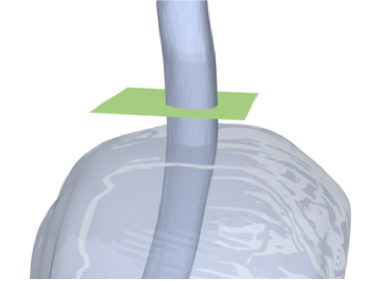
\includegraphics[width=.4\textwidth]{validation/cutPlane1}}\qquad\qquad
%   \subbottom[]{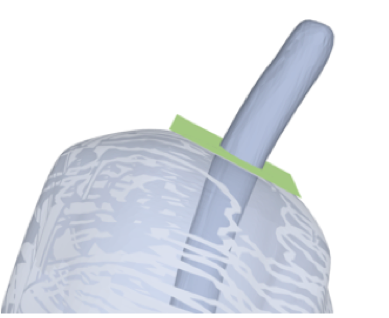
\includegraphics[width=.4\textwidth]{validation/cutPlane2}}
%   \caption{Good urethra cutting planes}
%   \label{fig:goodCutPlanes}
% \end{figure}

% \begin{figure}
%   \centering
%   \subbottom[]{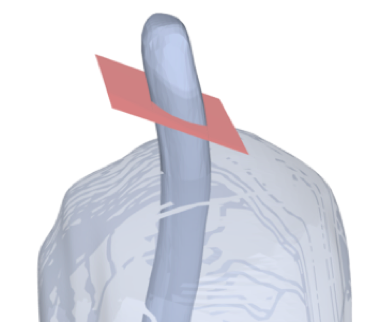
\includegraphics[width=.4\textwidth]{validation/B-cutPlane1}}\qquad\qquad
%   \subbottom[]{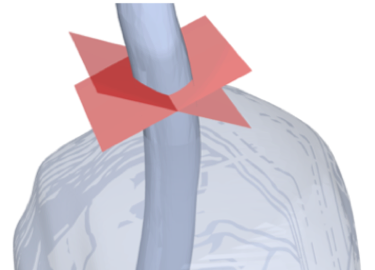
\includegraphics[width=.4\textwidth]{validation/B-cutPlane3}}
%   \caption{Bad urethra cutting planes}
%   \label{fig:badCutPlanes}
% \end{figure}

% 	\item \textbf{Size of the cut:} small snips at a time: A good practice for a clean cut is cutting only a few millimeters at a time. The size of a good cut is currently calculated by the surface area that has been separated.  If the surface area is above a certain threshold, it is considered a large cut. If it is below, it is considered a good cut. Having big snips may risk in cutting different layers that should not be cut like nerves. \autoref{fig:goodBadCuts} below show two different examples of big and small cuts.

% 	%snips
% \begin{figure}
%   \centering
%   \subbottom[]{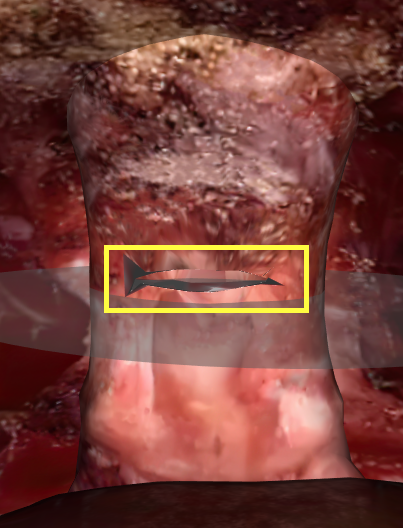
\includegraphics[width=.4\textwidth,frame]{validation/bigCut}}\qquad\qquad
%   \subbottom[]{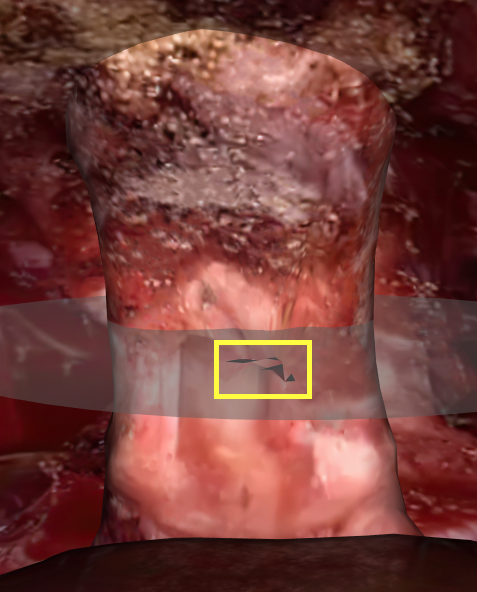
\includegraphics[width=.422\textwidth,frame]{validation/smallCut}}
%   \caption{(\emph{a}) shows an example of a bad cut, whereas (\emph{b}) shows an example of a good cut \ie small snip}
%   \label{fig:goodBadCuts}
% \end{figure}

% 	\item \textbf{Topological cut:} A good practice for a clean cut, the surgeon should perform the task starting from only one initial cut and continue along the same plane in the urethra and should not create multiple initial cuts. By the end of the simulation, there should exist one continuous cut around the urethra that separates it into two pieces. Whether the surgeon prefers to create one or multiple small cuts initially, they should end up as one eventually. To calculate topological cuts, once a cut is performed, we take a set intersection between the triangles of the mesh after cutting and the initial mesh. The result of this would be the new triangles resulting from all cuts. By counting the number of disjoint group of triangles, we can identify the number of topological cut. \autoref{fig:topCut} shows different snip sizes.

%   \begin{figure}
%     \centering
%     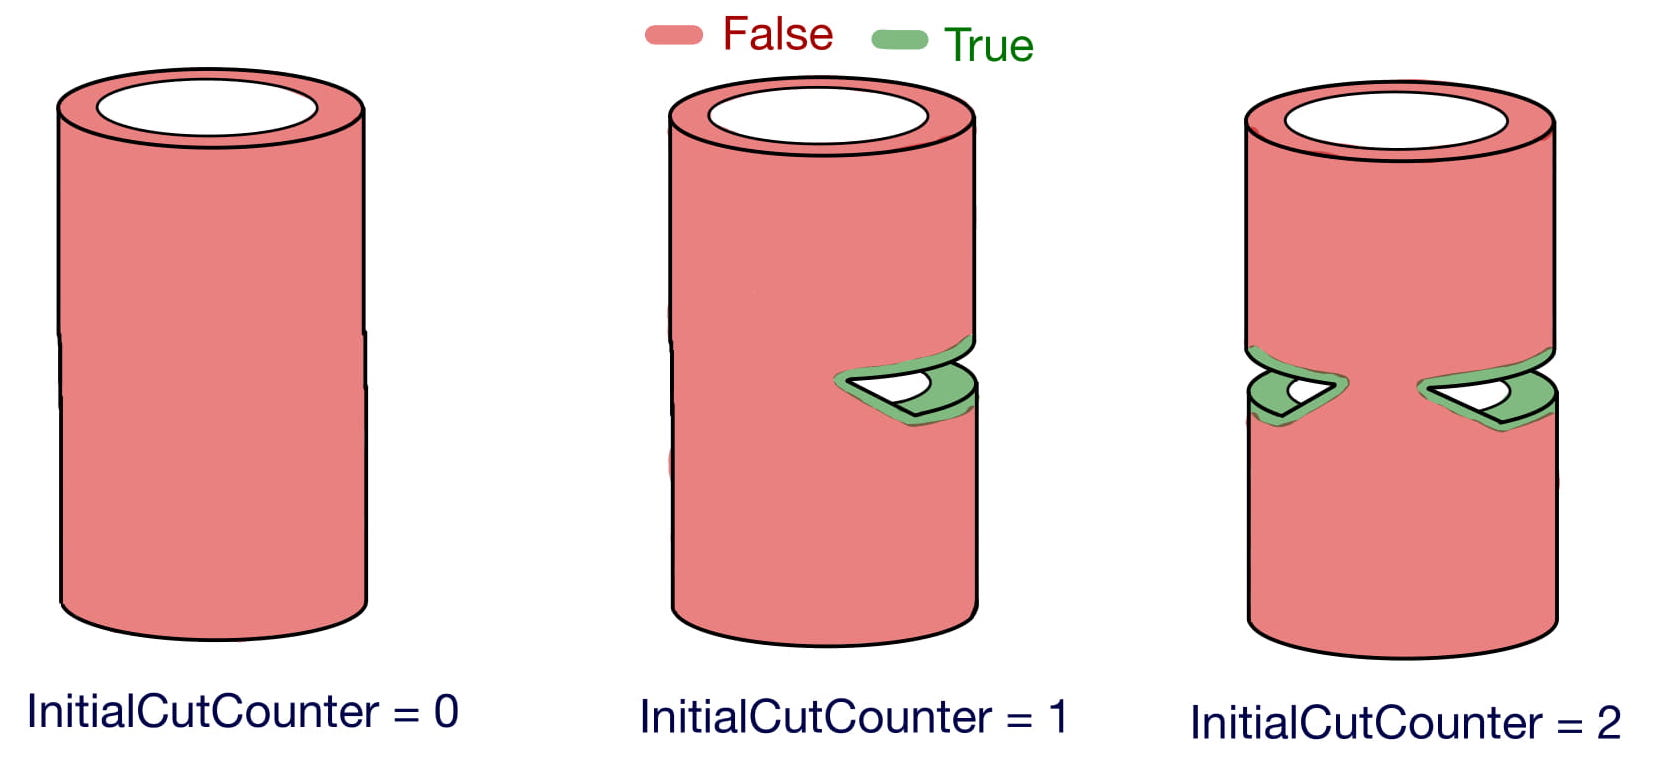
\includegraphics[width=.7\textwidth]{validation/initial_cut.jpg}
%     \caption{Cutting plane with multiple initial cuts. It ends up with only one topological cut}
%     \label{fig:topCut}
%   \end{figure}

% 	\item \textbf{Rectal wall collisions:} A good practice is to avoid collisions with the surrounding tissues and rectal wall. Injuries in the rectum occur more often during the dissection of the prostatic apex (if not completely mobilized off of the posterior of the prostate). When the rectum stays adherent to the apex, it is at a risk of injury in the process of urethra transecting. \autoref{fig:recWalls} below shows the rectal wall as white-shaded areas.

%   \begin{figure}
%     \centering
%     \subbottom[]{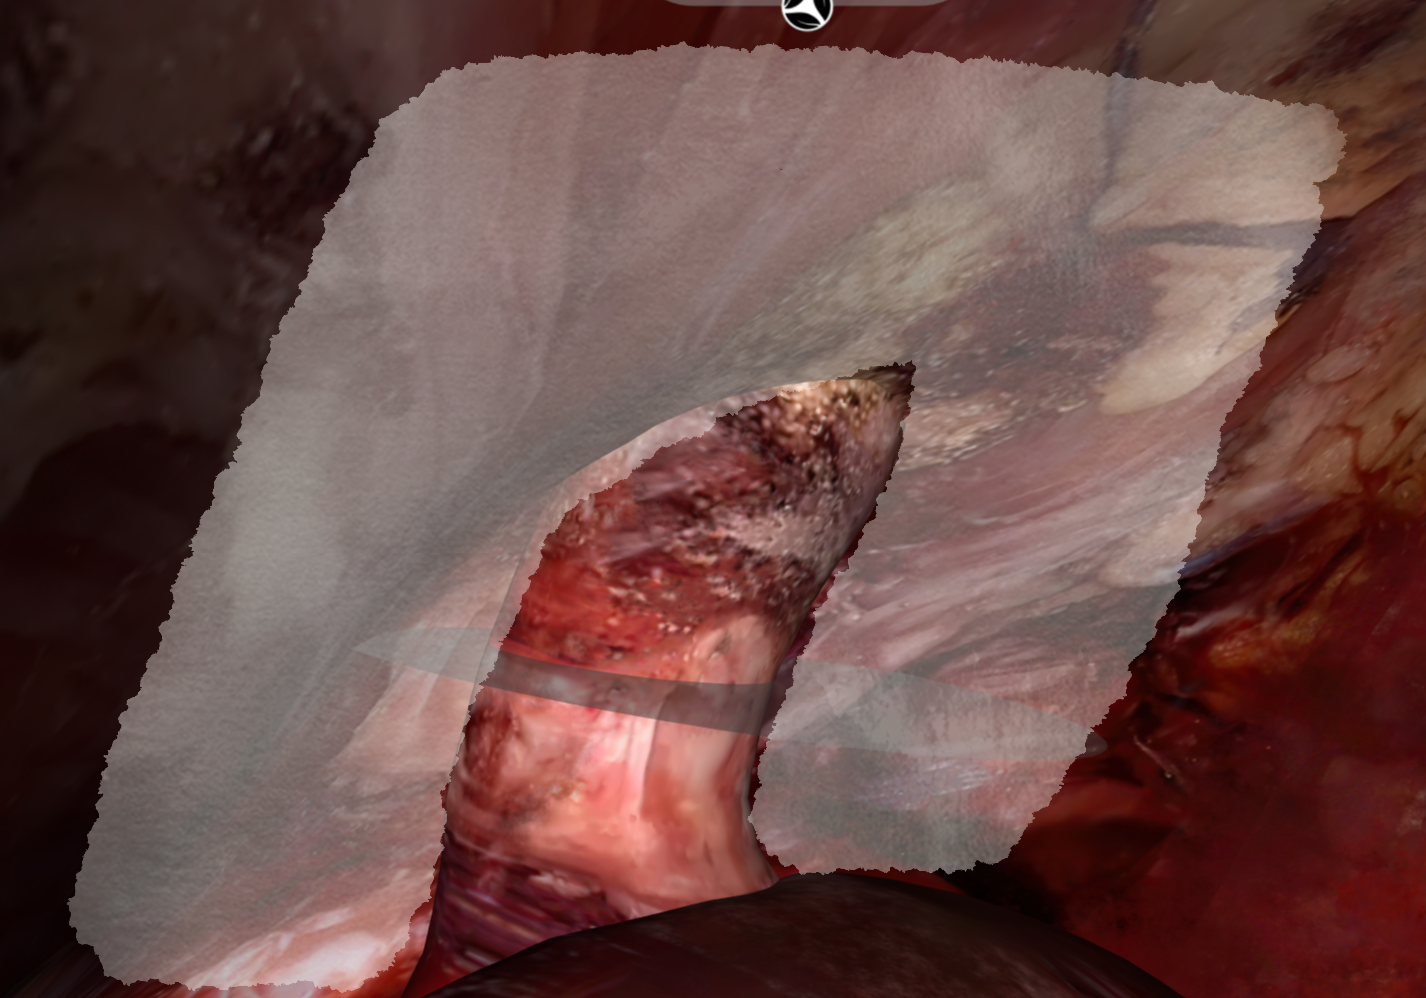
\includegraphics[width=.42\textwidth,frame]{validation/rec1}}\qquad
%     \subbottom[]{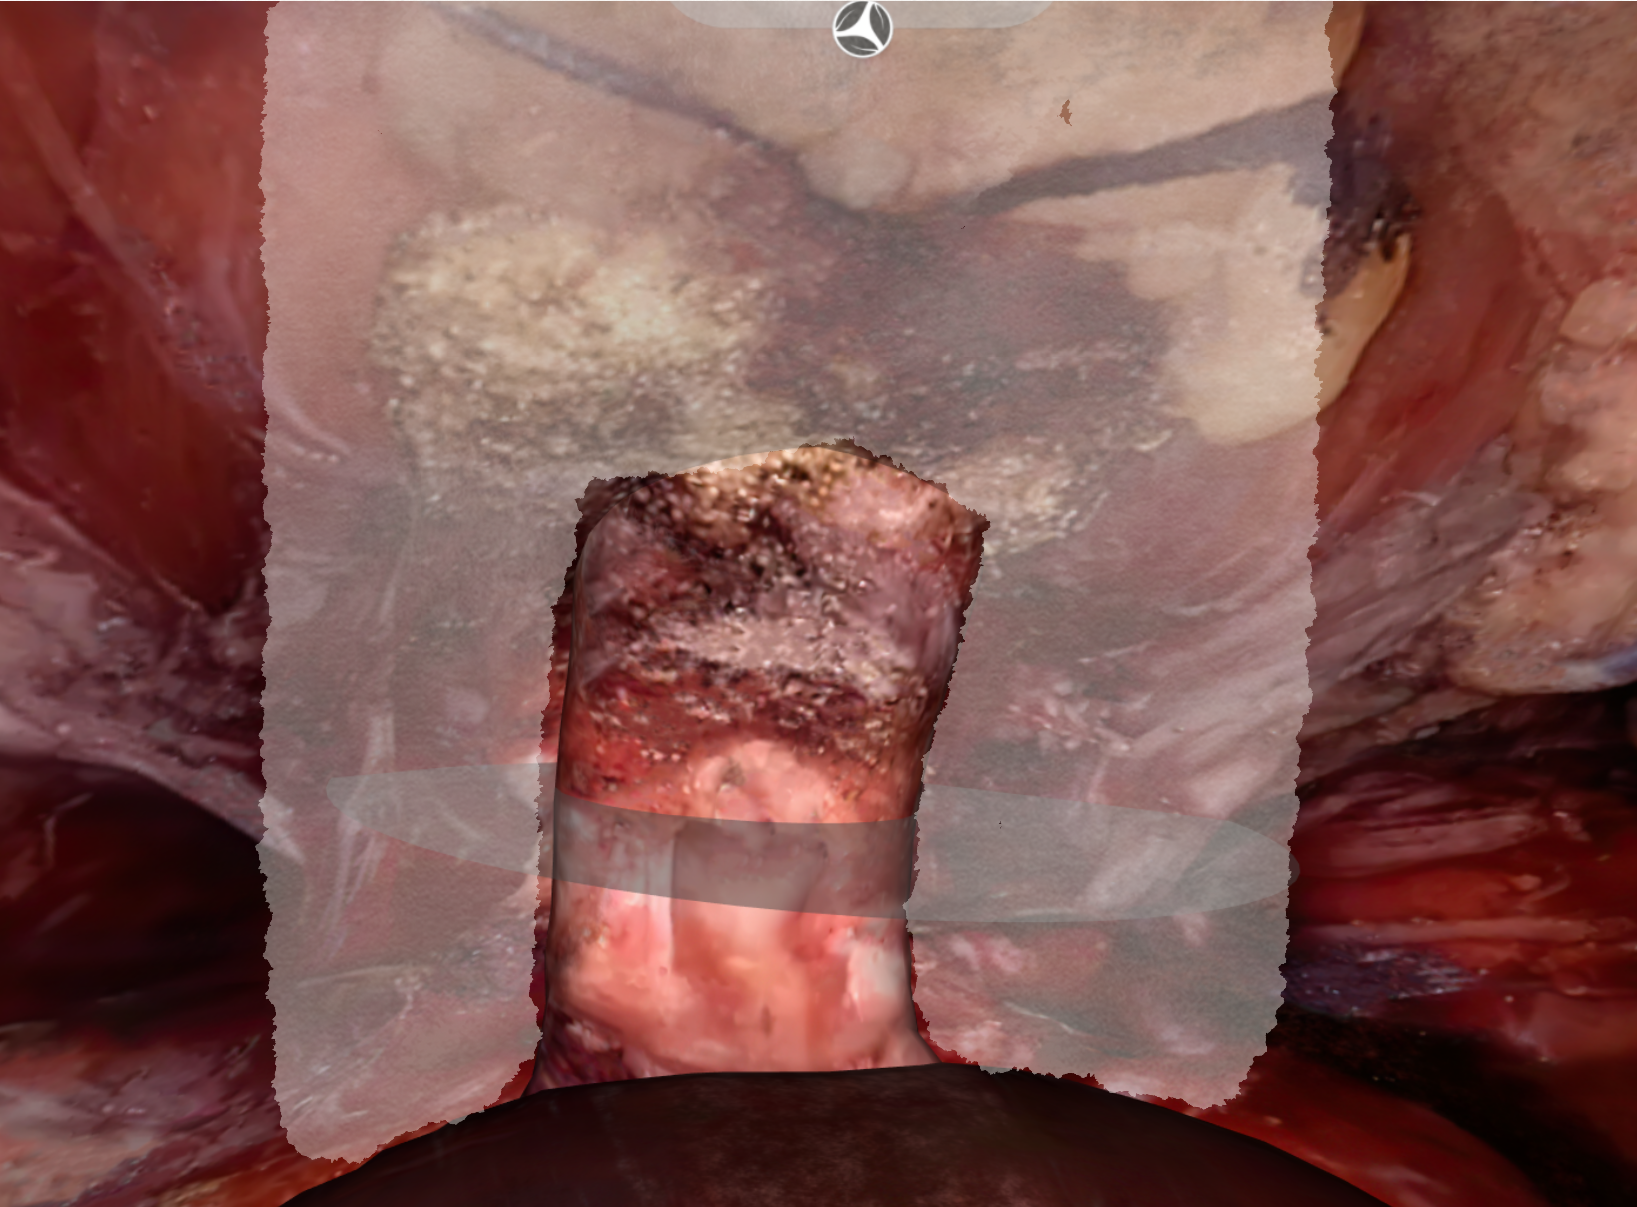
\includegraphics[width=.4\textwidth,frame]{validation/rec2}}
%     \caption{(\emph{a}) Side view of rectal wall boarders (\emph{b}) Front view of rectal wall boarders}
%     \label{fig:recWalls}
%   \end{figure}

% 	\item \textbf{Tools out-of-scene count:} A good practice is to keep surgical tools always visible within the surgical view. Moving the tools out of the scene may result in injuring the patient in a real operation setting. The surgeon shall be able to control the motion of these surgical tools and keep them within his surgical view. \autoref{fig:fov} illustrates the good and bad scenarios of this parameter.

%   \begin{figure}
%     \centering
%     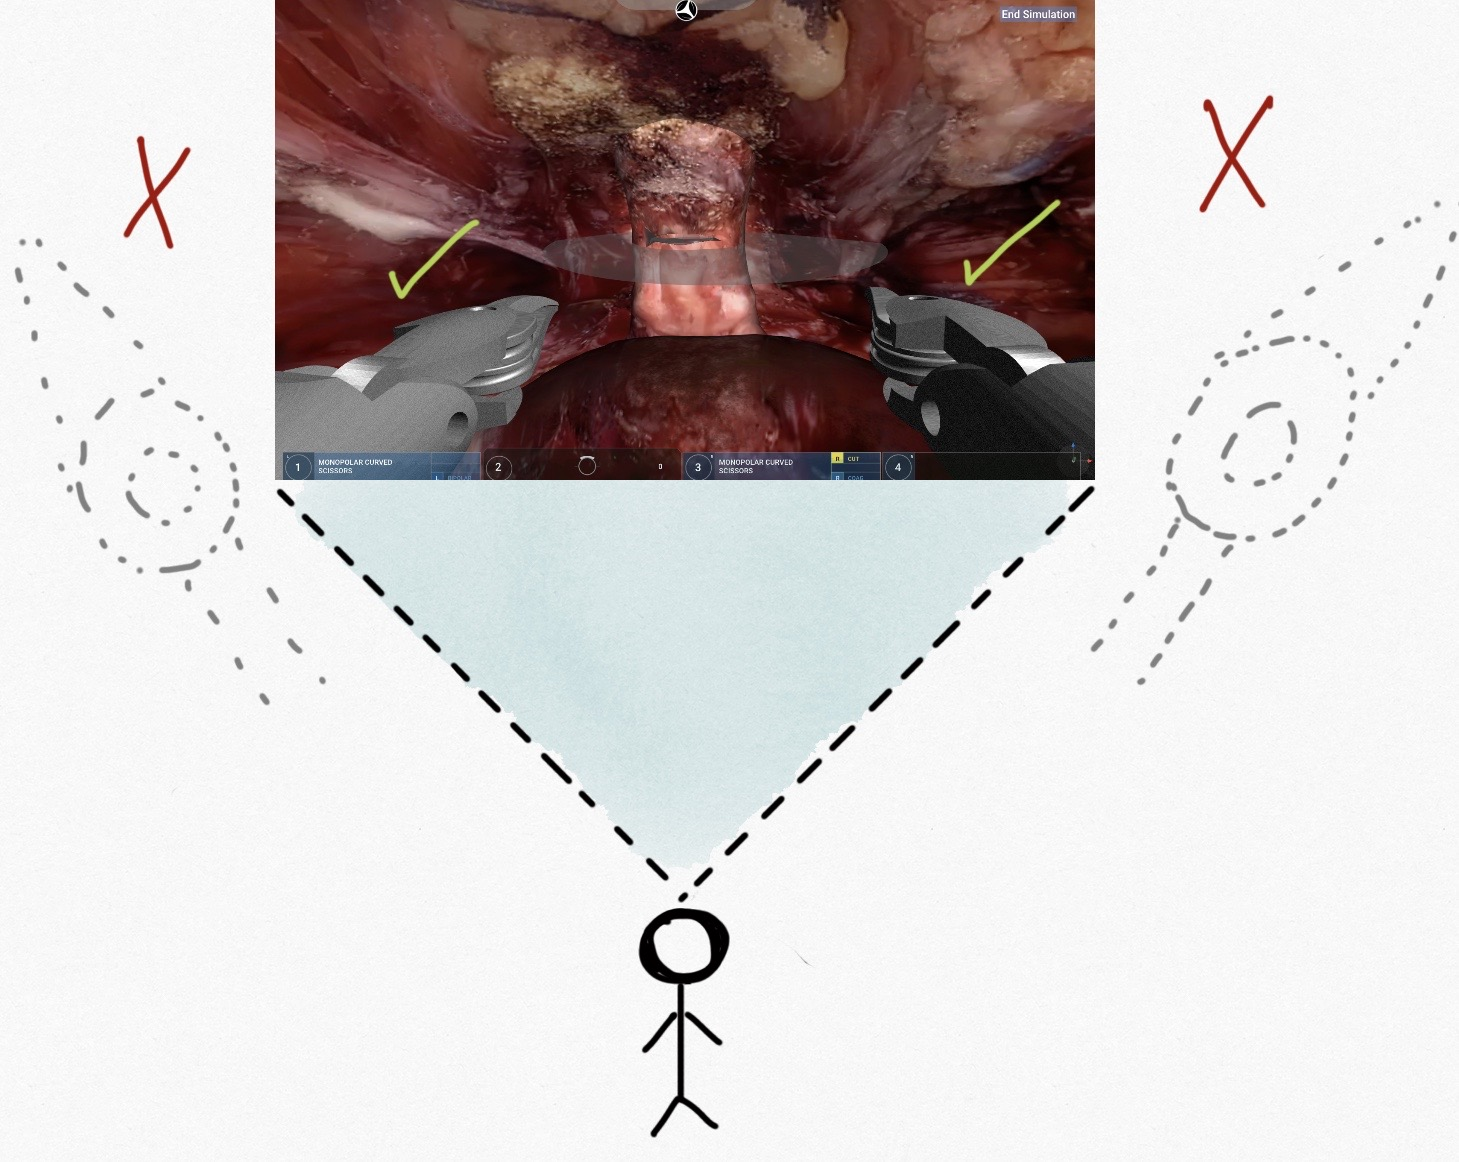
\includegraphics[width=.9\textwidth,frame]{validation/fov}
%     \caption{Tools should be always kept within the field of view. Tools out of the scene are dangerous in a real setting.}
%     \label{fig:fov}
%   \end{figure}
% 	\item \textbf{Time elapsed for task completion:} This parameter will be used to assess the skills acquired by surgeons by using this simulator through their difference in performance parameters throughout trials. This parameter will also be used as an indication to differentiate between different surgeon expertise: a senior surgeon who is used to the console setup performs the task faster than a novice surgeon.
% \end{enumerate}

\begin{sidewaystable}
%\begin{table}
\small
\centering
\begin{tabular}{m{1.2cm}m{3.2cm}m{9cm}m{6.5cm}}
  \multicolumn{2}{c}{\text{Parameter}} & How it is computed? & Sample data\\
  \toprule
  Para \#1 & Plane of the cut & Storing the angle between ideal plane of cut and tooltip upvector & Cut-1: \SI{5}{\degree} \newline Cut-2: \SI{23}{\degree} \newline \ldots \newline Cut n: \SI{10}{\degree}\\
  \midrule
  Para \#2 & Size of the cut & Storing the summation of the area of the new surface introduced by the cut & Cut 1: \SI{5}{\metre\squared} \newline Cut 2: \SI{10}{\metre\squared} \newline \ldots \newline Cut n: \SI{3}{\metre\squared}\\
  \midrule
  Para \#3 & Topological cuts & Storing disconnect pairs of triangle soup & Cut 1: 1 topological cut \newline Cut 2: 2 topological cut \newline \ldots \newline Cut n: 1 topological cut\\
  \midrule
  Para \#4 & Rectal Wall Collision & Setting counter for tooltip to pass a plane representing rectal wall & Before Cut 1: 0 rectal wall collisions \newline Before Cut 2: 1 rectal wall collisions \newline \ldots \newline Before Cut n: 0 rectal wall collisions\\
  \midrule
  Para \#5 & Tools out-of-scene count & Using projection matrix & Before Cut 1: 0 tooltips out of surgical view \newline Before Cut 2: 1 tooltips out of surgical view \newline \ldots \newline Before Cut n: 0 tooltips out of surgical view\\
  \midrule
  Para \#6 & Total time for task completion & Storing time stamps & Till Cut 1: \SI{6}{\second} \newline Till Cut 2: \SI{24}{\second} \newline \ldots \newline Till Cut n: \SI{187}{\second}\\
  \bottomrule
\end{tabular}
\caption{Parameters collected during the construct validity}
\label{tab:params}
%\end{table}
\end{sidewaystable}

\begin{table}
\small
\centering
\begin{tabular}{c}
 Log file (CSV format) generated for a user trial\\
 \toprule
 Cut-1: Para \#1, Para \#2, Para \#3, Para \#4, Para \#5, Para \#6 \\
 \midrule
 Cut-2: Para \#1, Para \#2, Para \#3, Para \#4, Para \#5, Para \#6\\
 \midrule
 \ldots\\
 \midrule
 Cut-$n$: Para \#1, Para \#2, Para \#3, Para \#4, Para \#5, Para \#6\\
 \bottomrule
\end{tabular}
\caption{Sample output format}
\label{tab:csv}
\end{table}

\section{Data Analysis}
Upon performing the construct validity, we are able to quantify the subjects performance across trials and access how good is the simulator assessing their current performance and giving them feedback that would improve it in the next trial. As mentioned above, subjects were asked to perform 5 trials.

To analyse data, we have visualized the recorded parameters per trial as a first step and then aggregated all trials of all subjects to assess their overall performance. For each of the subjects, it is clear that they are reflecting from their previous mistakes from the mini on-screen report that they see by the end of each trial. For almost all trials, all subjects have successfully decreased the number of mistakes in the following trial. Therefore, the on-screen report is crucial for performance feedback and improvement purposes.

The figures below show the performance of the subjects in terms of:
\begin{enumerate}
    \item \textbf{Topological cuts:} Topological cuts by the end of the simulation would be at most 1. In some of the trials, some subjects had more than one. They were learning progressively.
    \item \textbf{Tools out of scene count:} Tools should remain with the surgical view. When the tools are out of the scene, the subject is visually notified and prompted to remain within the scene boundaries. The count is eventually displayed in the on-screen report.
    \item \textbf{Rectal wall collisions count:} Tools should not be touching the surrounding organs. When the tool touches the rectal wall, the subject is visually notified and prompted to not touch it. The number of hits is shown in the on-screen report in the end of the simulation.
\end{enumerate}

A list of plots in \autoref{fig:indivSubjs} shows all trials and for all subjects.

\begin{figure}
  \centering
  \subbottom[]{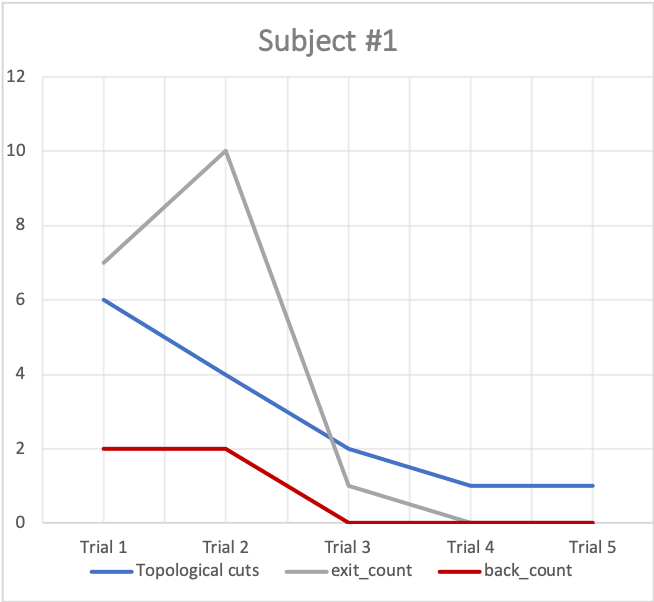
\includegraphics[width=.4\textwidth]{validation/sub1}}\qquad
  \subbottom[]{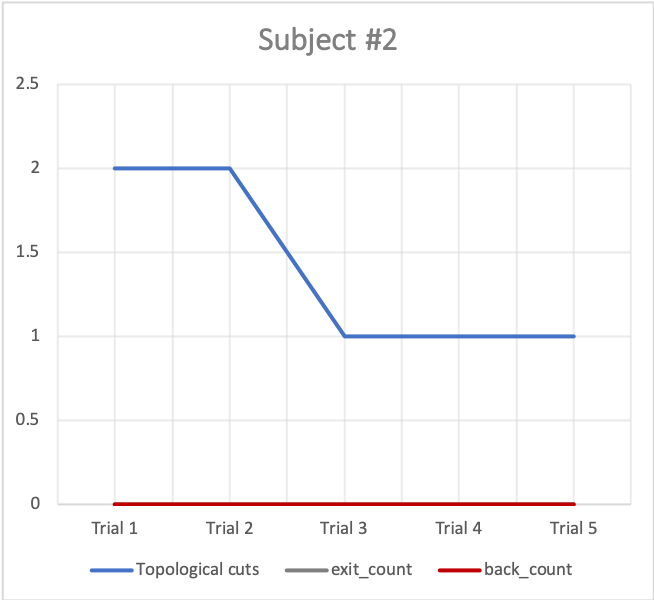
\includegraphics[width=.4\textwidth]{validation/sub2}}\qquad\\
  \subbottom[]{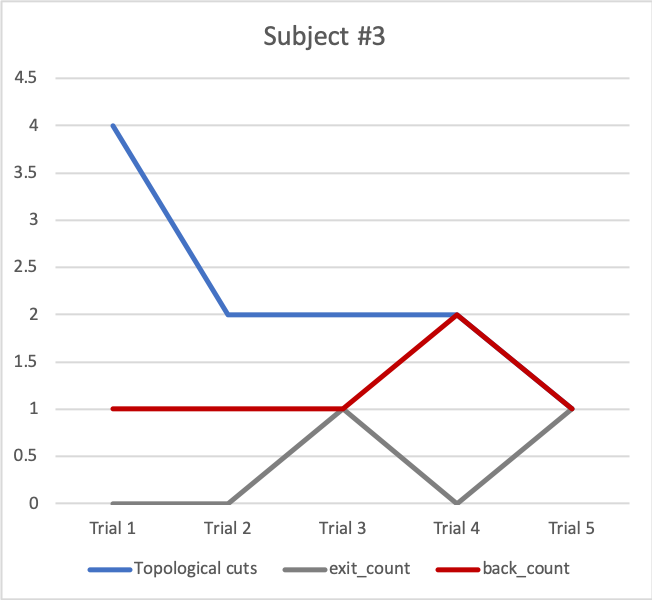
\includegraphics[width=.4\textwidth]{validation/sub3}}\qquad
  \subbottom[]{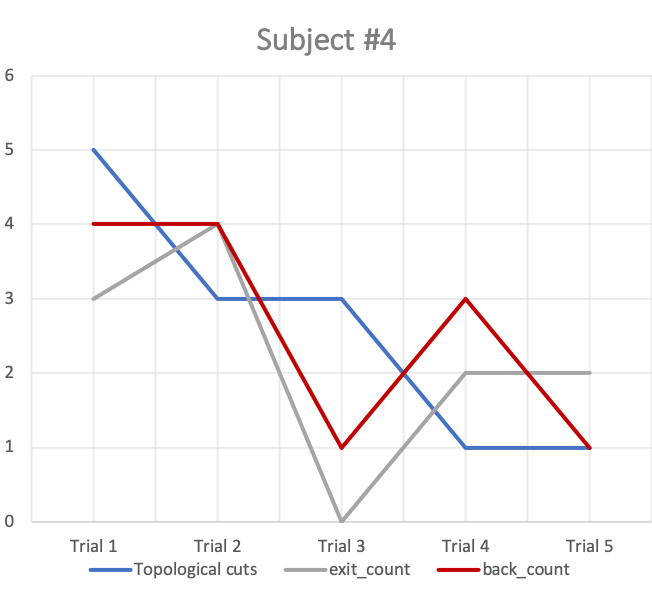
\includegraphics[width=.4\textwidth]{validation/sub4}}\qquad\\
  \subbottom[]{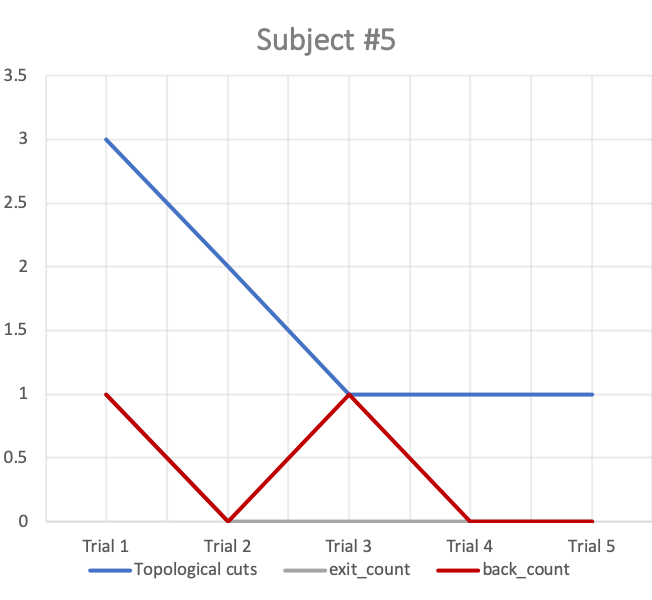
\includegraphics[width=.4\textwidth]{validation/sub5}}\qquad
  \subbottom[]{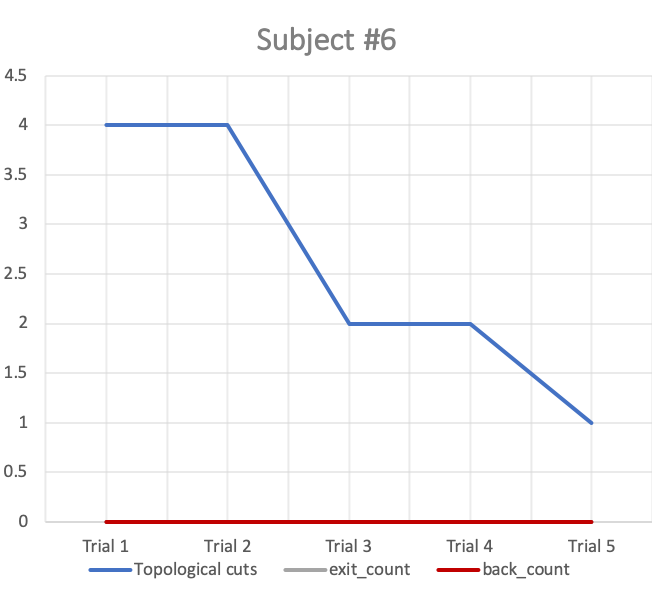
\includegraphics[width=.4\textwidth]{validation/sub6}}
  \caption{(\emph{a}) Subject 1 performance on three parameters: topological cuts, tools out of scene count, and rectal wall hits count (\emph{b}) Subject 2 performance on the aforementioned parameters. Gray and red lines are identical. Hence, the missing gray line (\emph{c}) Subject 3 performance on the aforementioned parameters (\emph{d}) Subject 4 performance on the aforementioned parameters (\emph{e}) Subject 5 performance on the aforementioned parameters (\emph{f}) Subject 6 performance on the aforementioned parameters. Gray and red lines are identical, hence the missing gray line.}
  \label{fig:indivSubjs}
\end{figure}

Variability of topological cuts data across trials in \autoref{fig:topcutvar} among all subjects is decreasing as subjects are performing more trials. This indicates that the on-screen mini-report they are receiving by the end of the trials is effective and communicates necessary information needed to have better performance in the next trial. This is further emphasized on \autoref{tab:contentTable2} through high mean values.

\begin{figure}
  \centering
  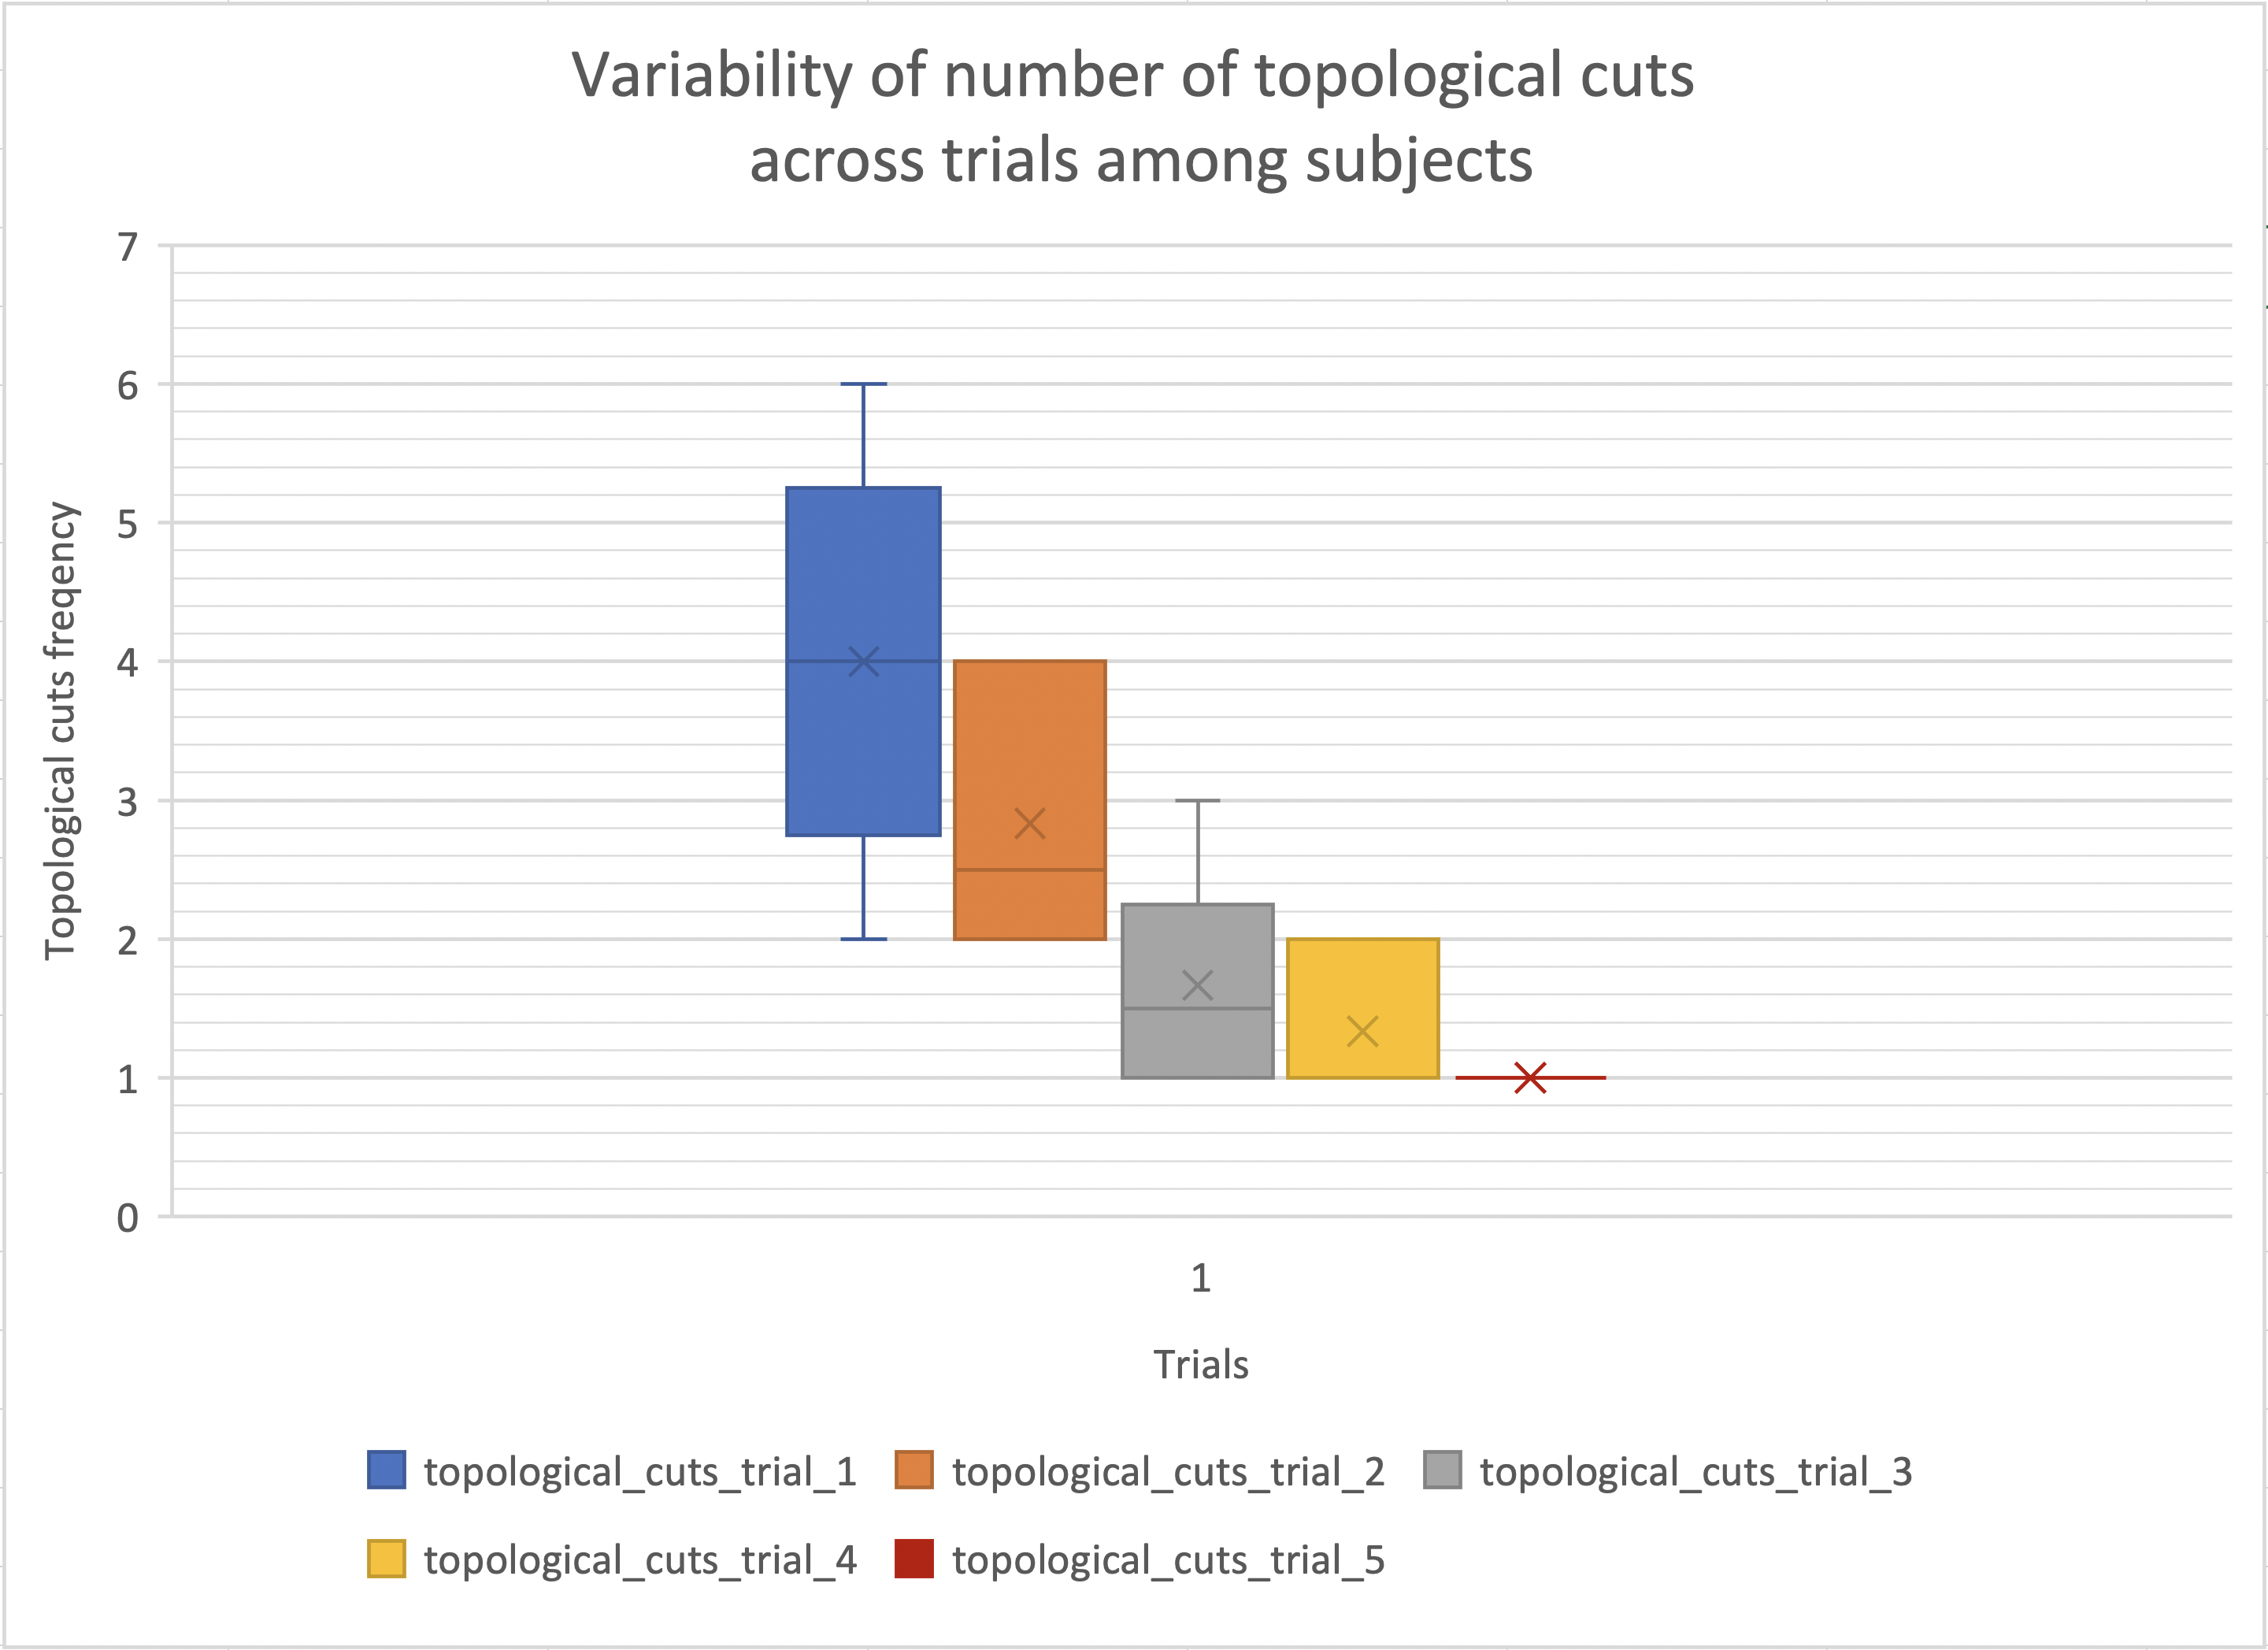
\includegraphics[width=.72\textwidth]{validation/topCutsVar}
  \caption{Variability of number of topological cuts across trials among subjects}
  \label{fig:topcutvar}
\end{figure}

Variability in the exit count data across trials in \autoref{fig:exitvar} shows high exit count values during early trials. This count drops significantly starting from the third trial onward. This signifies that live feedback upon scene exit and the generated on-screen mini report effectively communicates the user their performance as they are trying to reduce the count as low as possible in the next trials.

\begin{figure}
  \centering
  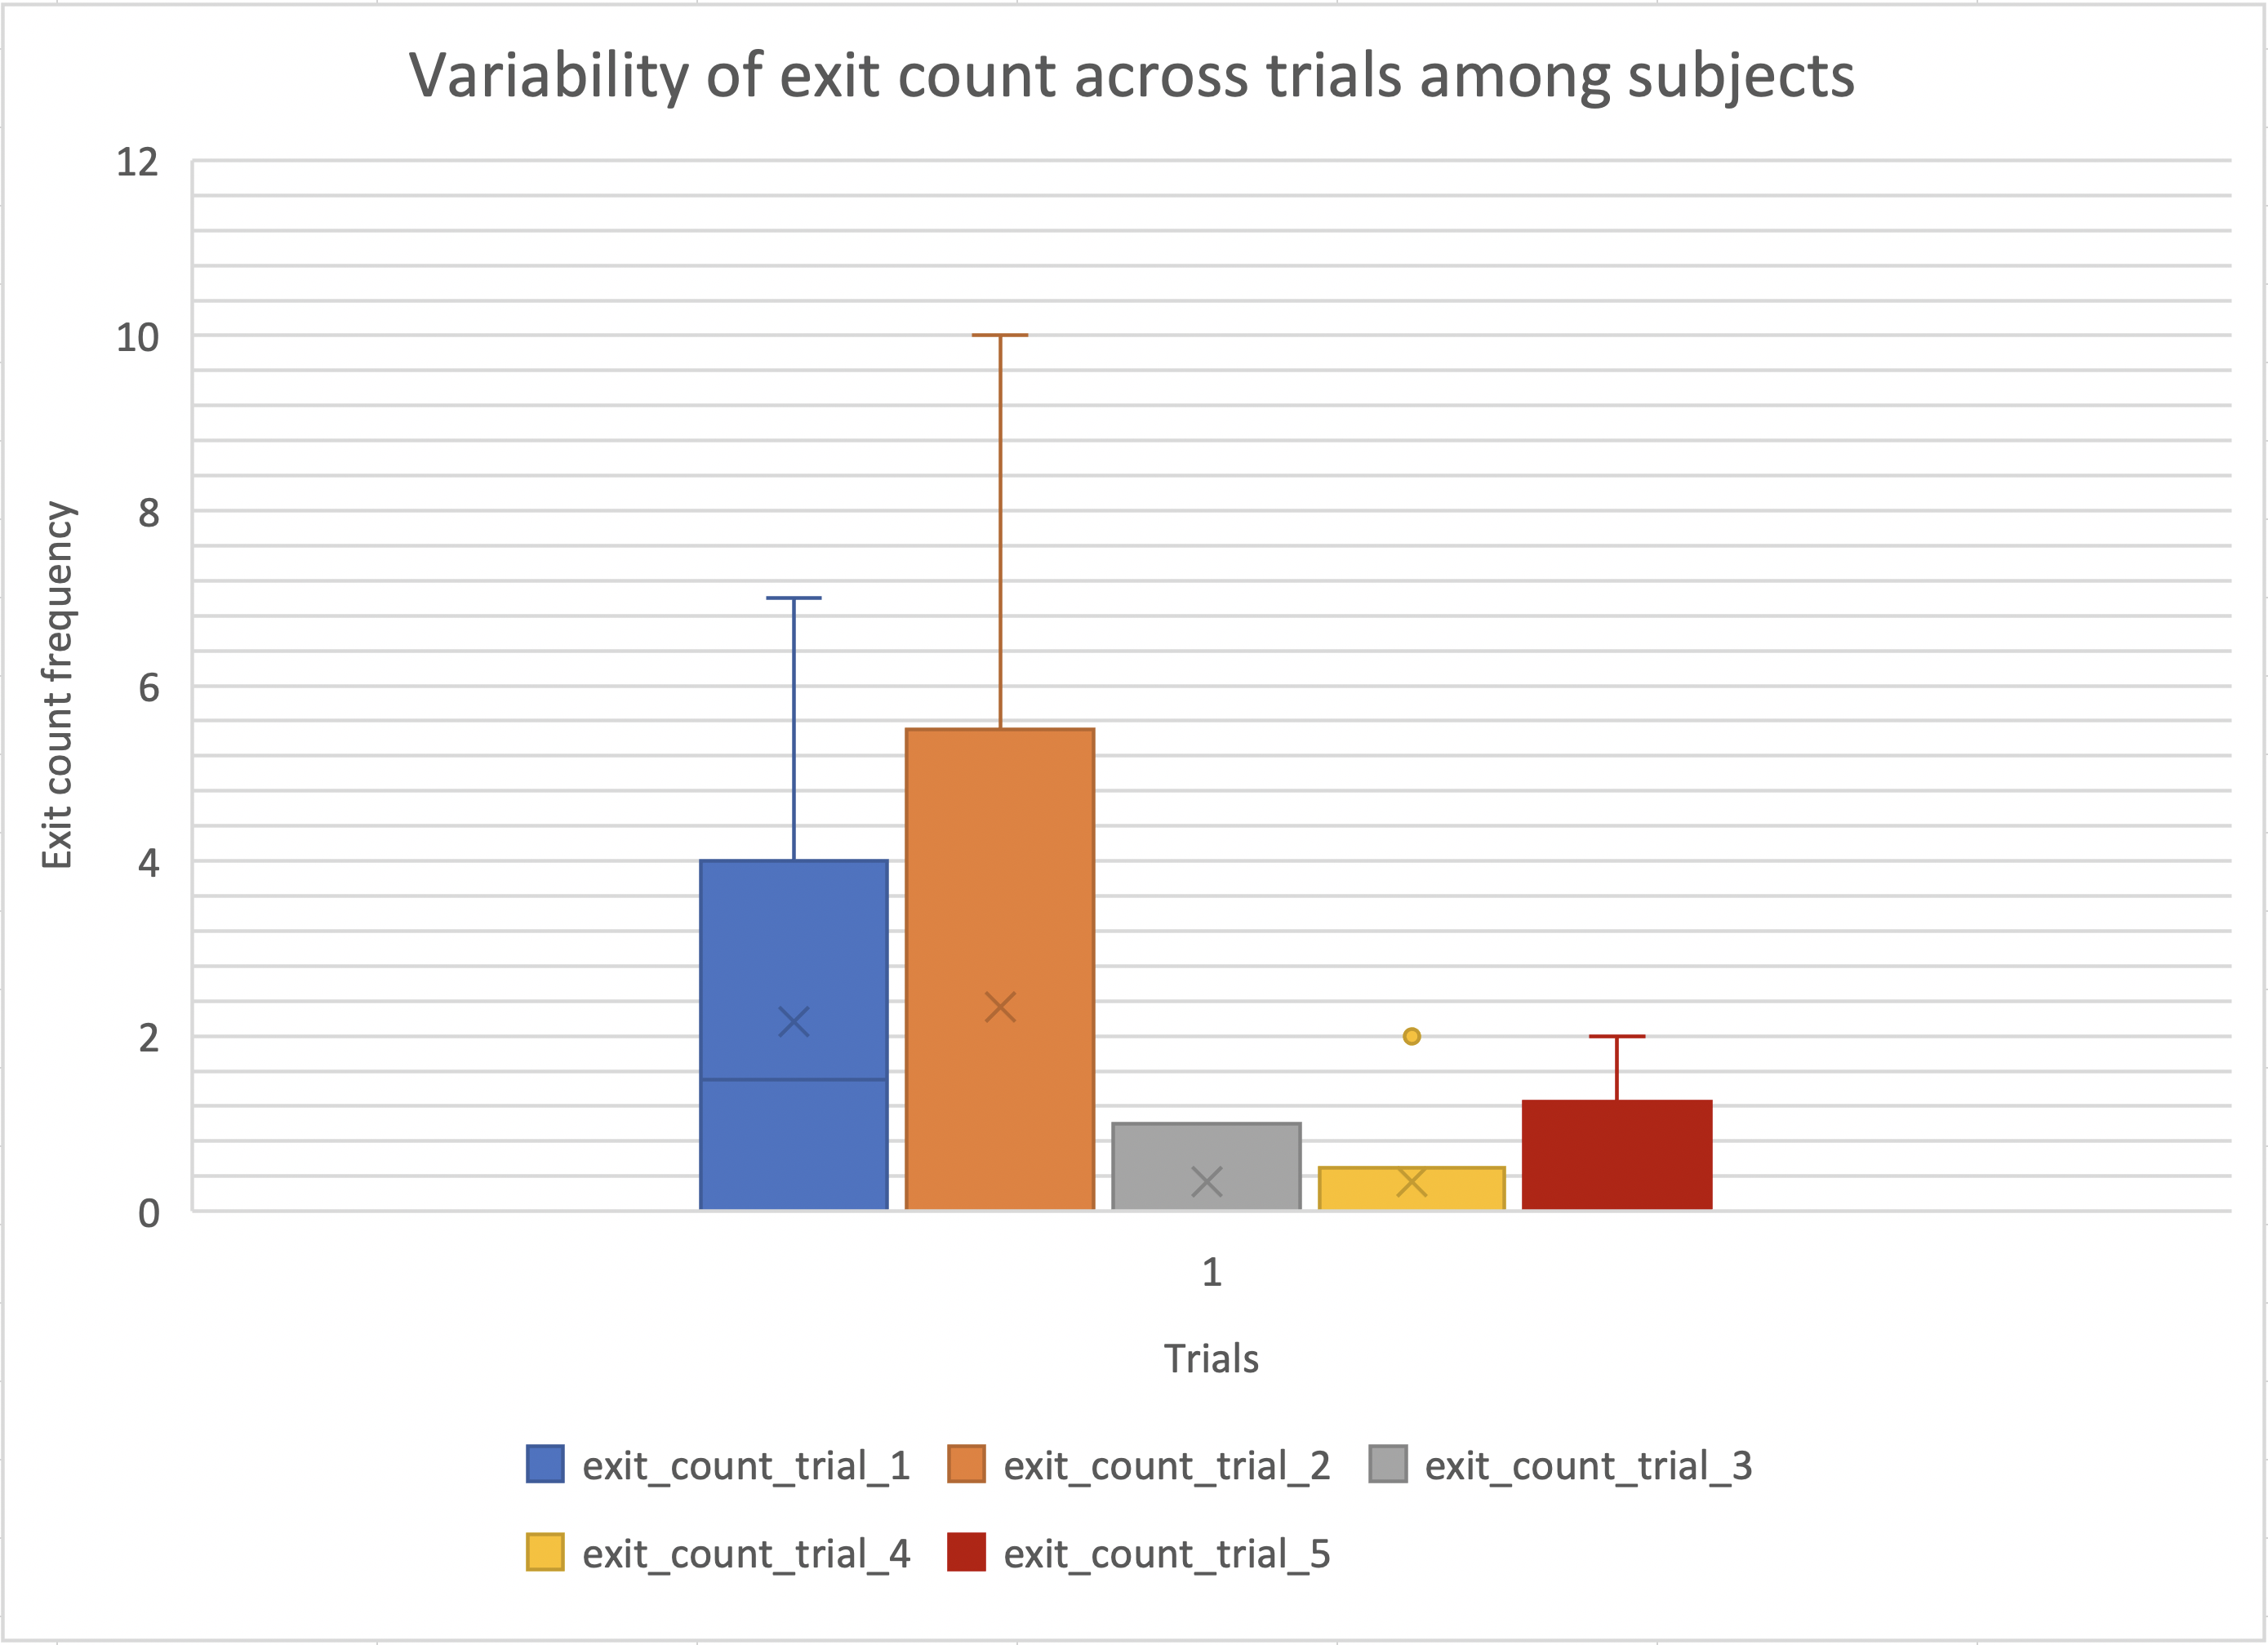
\includegraphics[width=.72\textwidth]{validation/exitCountVar}
  \caption{Variability of exit count across trials among subjects}
  \label{fig:exitvar}
\end{figure}

Variability in the rectal wall collision data in \autoref{fig:recwallvar} is not stable. This is mainly due to the dimensional constraint: during validation studies and when subjects are trying to reach the urethra to cut it, they often hit the rectal wall by mistake. This happens because they are not perceiving scene depth correctly. Hence, they tend to hit the rectal wall, thinking they did not reach the urethra yet. Almost all subjects come to consensus on this point. One subject suggested adding another view (top view for example) to be able to locate the tools, which is a feasible solution in a 2-dimensional display monitor without the need for extra hardware. Other solutions are using a stereoscopic display (3D or VR) or a holographic display to be able to perceive depth.

Another potential reason is the size of surgical tools: One of the dominant feedback we received is that the tools are too big in the scene and they are not as big in a real setting. As the tool is big, hitting the rectal wall shall happen often. A combined factor of big surgical tools and depth mis-perception significantly increased the chances of rectal wall collisions. To rectify this, the tools will be made smaller than the current size in the future versions of the simulator.

Taking by the subjects feedback, the depth issue was fixed by developing two different solutions and to check
\textbf{ADD ANOTHER SECTION FOR COMPARISON BETWEEN LKG AND VR}

Hypothesis: VR is better than LKG since it mimics a real DaVinci console.

Evaluation: pending
Analysis: using Chi-squared for significance testing.
Final summative feedback: Pass testing (yes or no)

\begin{figure}
  \centering
  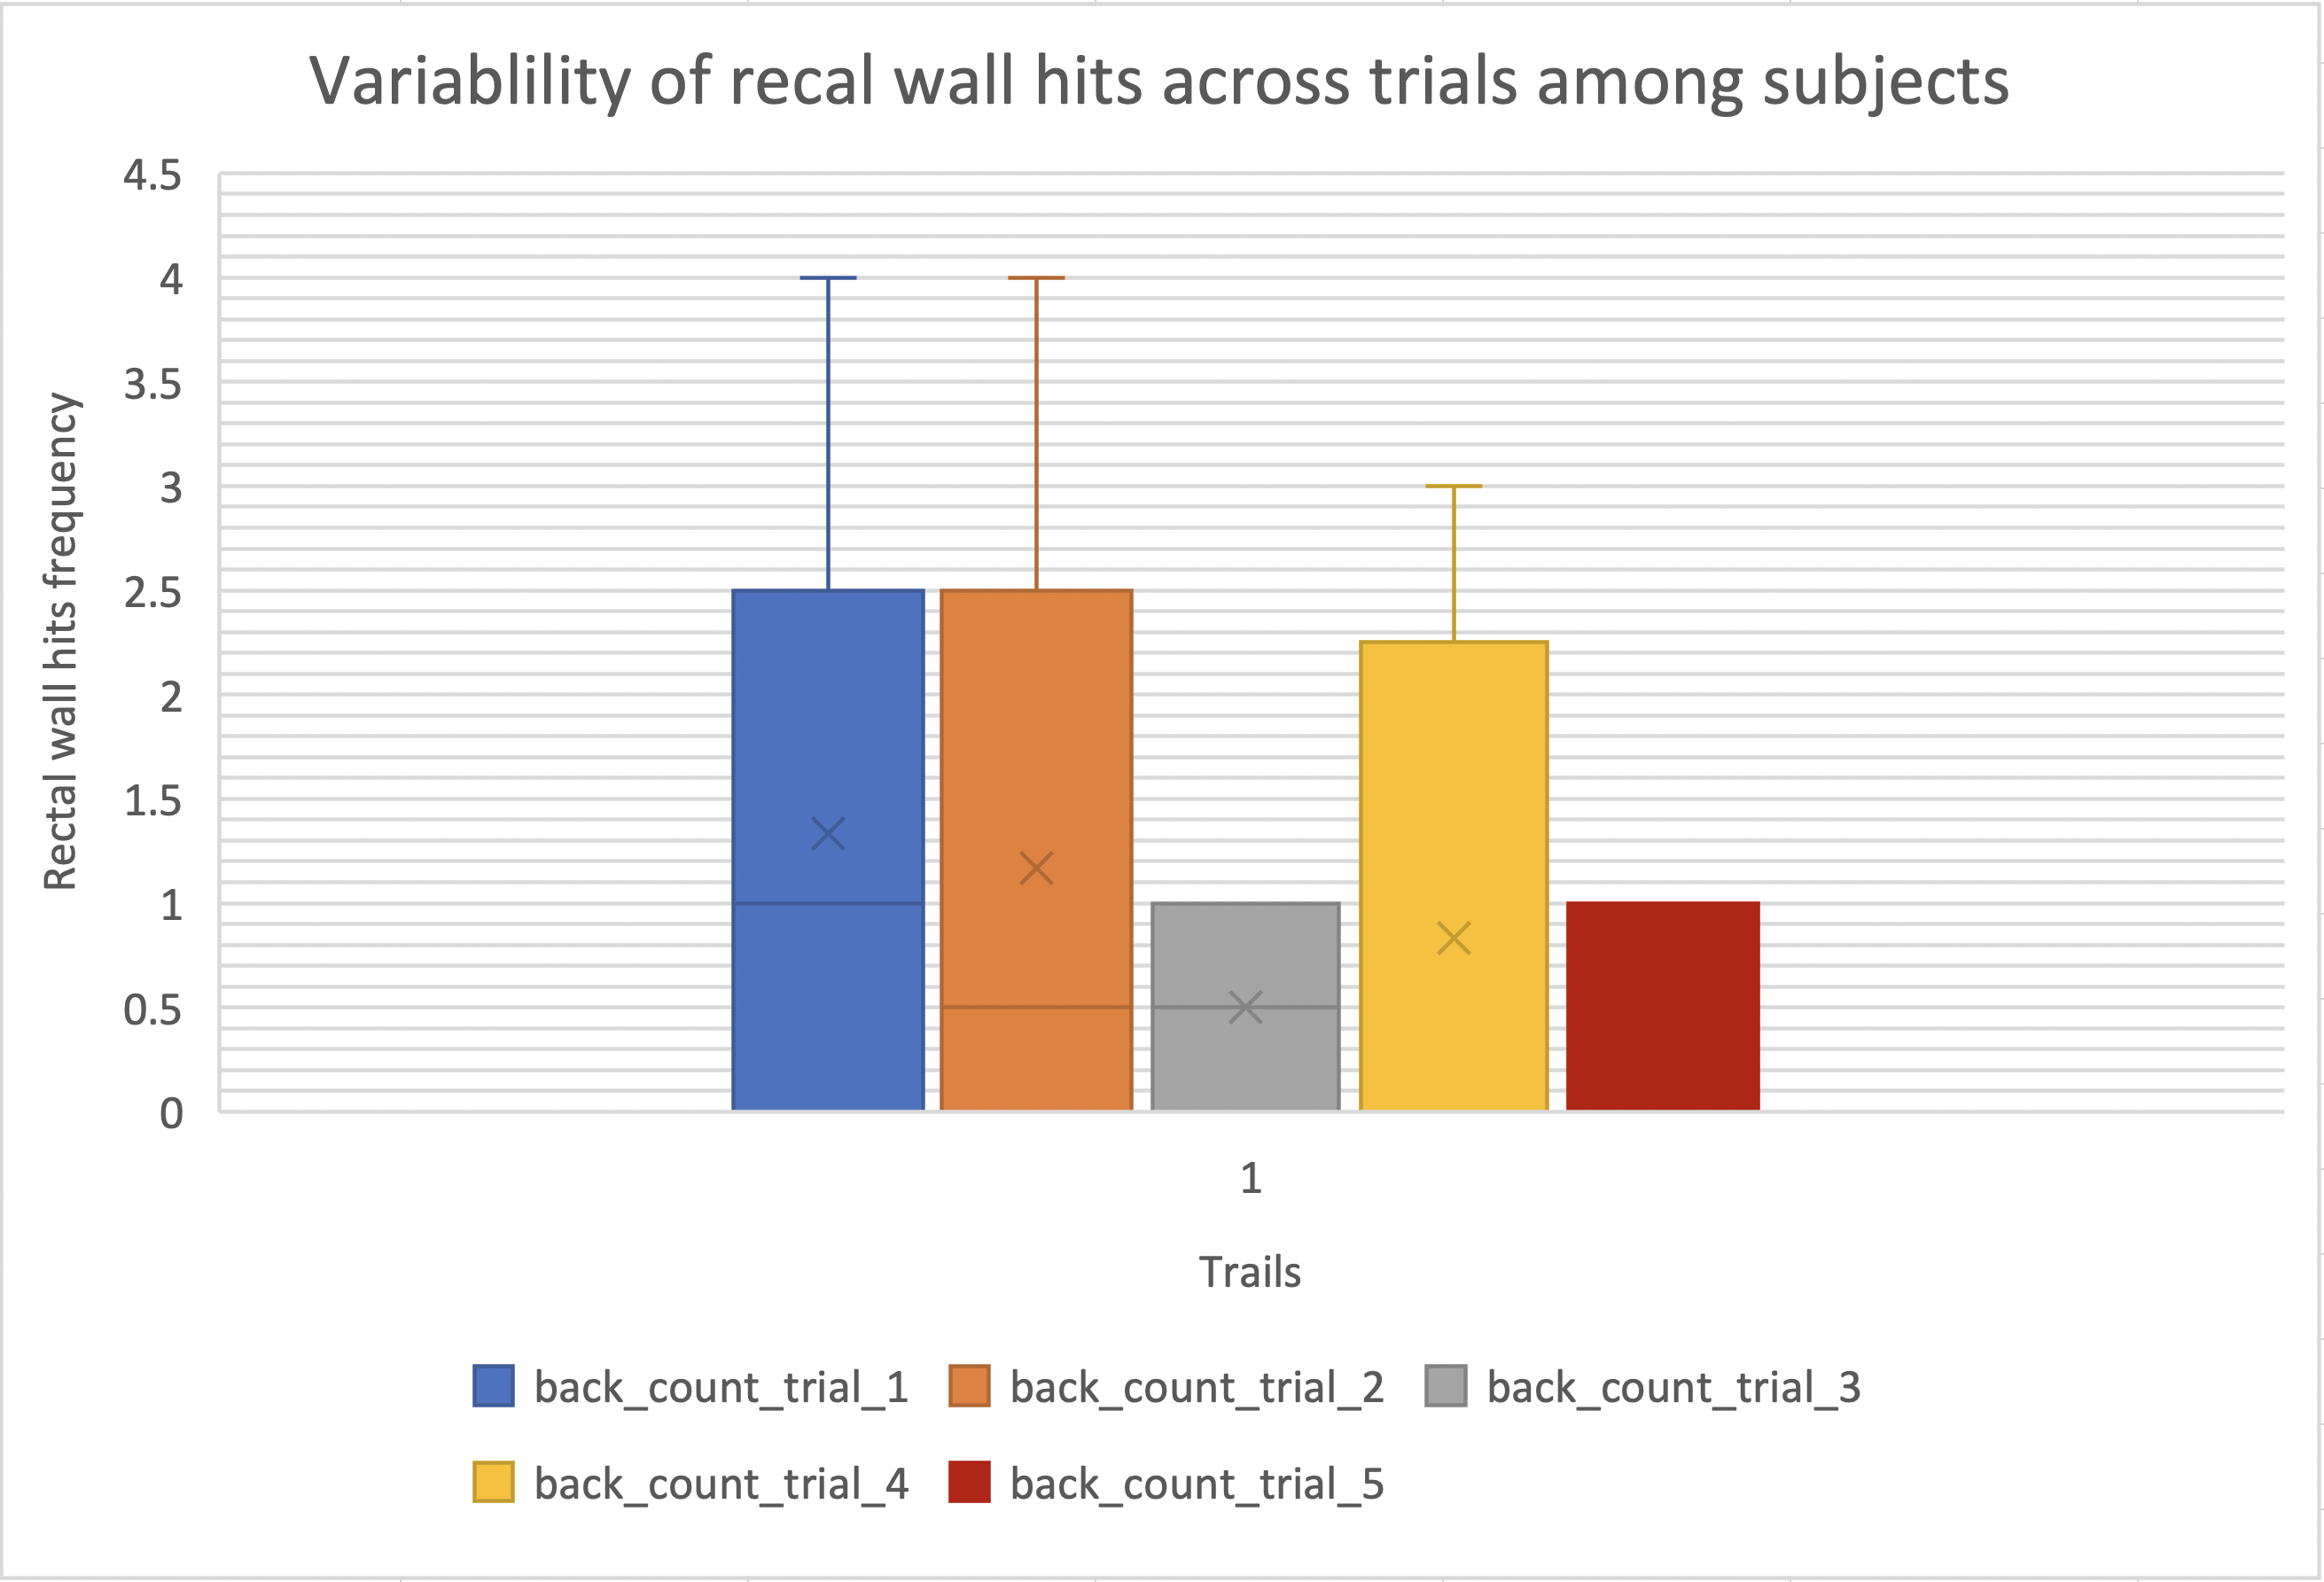
\includegraphics[width=.72\textwidth]{validation/recWallVar}
  \caption{Variability of rectal wall collisions count across trials among subjects}
  \label{fig:recwallvar}
\end{figure}

